  \documentclass[10pt,xcolor=table]{beamer}

\usepackage{graphicx}
\usepackage{caption}
\usepackage{subcaption}
\usepackage{transparent}
 \usepackage{amsmath}
 
% \usepackage[utf8]{inputenc}
% \usepackage[T1]{fontenc}
\usepackage[table]{xcolor}    % loads also »colortbl« 
%  \usepackage{enumitem}
\usepackage{ucltemplate}
\usepackage{color}

\usepackage{pgfgantt} % for grantt charts
\usepackage{rotating}
\usepackage[graphicx]{realboxes}

\usepackage{rotating}

\usepackage{tikz}
\usetikzlibrary{arrows,positioning, shapes.symbols,shapes.callouts,patterns,shapes,chains,calc,backgrounds,fadings}


\DeclareMathOperator*{\argmin}{arg\,min}
\DeclareMathOperator*{\argmax}{arg\,max}

% \definecolor{parCol}{rgb}{0.1, 0.1, 1}
% \definecolor{stCol}{rgb}{0.1, 0.6, 0.1}
% \definecolor{bothCol}{rgb}{0, 0.5, 0.5}

\definecolor{parCol}{rgb}{0, 0, 0}
\definecolor{stCol}{rgb}{0, 0, 0}
\definecolor{bothCol}{rgb}{0, 0, 0}
 
%Information to be included in the title page:
\title{User Case Study 2: University College London Hospitals - Biomedical Research Centre}
\author{Razvan Valentin Marinescu}
\institute{Supervisors: Daniel C. Alexander, Sebastian Crutch}
\date{}

% logo of my university

\titlegraphic{
  \hspace{-4em}
   \begin{figure}
%    \centering
   \begin{subfigure}{0.20\textwidth}
   \hspace{2em}
   \includegraphics[height=0.8cm]{epsrc_logo.jpg}
   \end{subfigure}
   \begin{subfigure}{0.20\textwidth}
   \centering
   \includegraphics[height=0.8cm]{NEWpond2017b.png} 
   \end{subfigure}
   \begin{subfigure}{0.20\textwidth}
   \centering
   \includegraphics[height=0.8cm]{pondLogo.png} 
   \end{subfigure}
   \begin{subfigure}{0.20\textwidth}
   \centering
   \includegraphics[height=0.8cm]{brcLogo.jpg} 
   \end{subfigure}
   
   
   \end{figure}
}
 
 
\setbeamersize{text margin left=15pt,text margin right=15pt}


\begin{document}
 
\frame{\titlepage}
 
\setbeamerfont{frametitle}{size=\large}

% Presentation 9minutes in length + 3 min Q/A

\begin{frame}
\frametitle{About me}

\begin{itemize}
 \item Born and raised in Pitesti, Romania
 
  \begin{figure}
%   \right 
  \vspace{1em}
  \includegraphics[height=3cm]{pitestiRomania}\hspace{1em}\includegraphics[height=3cm,trim=0 0 0 100,clip]{bratianu}
  \end{figure}
 
 \vspace{1em}
 \item 2010-2014: Studied MEng in Computer Science at Imperial College
 
 \item 2014: Joined the EPSRC CDT in Medical Imaging at UCL
 \vspace{1em}
 \begin{figure}
 \centering 
 \includegraphics[height=1.0cm]{NEWpond2017b.png} \hspace{2em} \includegraphics[height=1.0cm]{logoImperial}  
 \end{figure}

\end{itemize}



\end{frame}


\begin{frame}
\frametitle{Why the CDT?}

\begin{itemize}
 \item Daniel Ruckert from Imperial College recommended me to apply

 \vspace{1em}
 
 \item I liked the idea of working in a multi-disciplinary environment that combines:
 
 \begin{figure}
  \begin{subfigure}{0.29\textwidth}
  \centering 
  computer science
   \includegraphics[height=1.6cm,trim=300 0 0 0,clip]{computerScience}
  \end{subfigure}
  \begin{subfigure}{0.29\textwidth}
  \centering 
  mathematics
   \includegraphics[height=1.6cm]{mathematics.jpg}
  \end{subfigure}
  \begin{subfigure}{0.29\textwidth}
  \centering 
  medicine
   \includegraphics[height=1.6cm]{medicine.jpg}
  \end{subfigure}
 \end{figure}

 \vspace{1em}
 
 \item Help solve some of the most devastating diseases worldwide
 
 \begin{figure}
 \centering
 \includegraphics[height=2.5cm]{adPrevalence}
 
 \end{figure}

 
\end{itemize}

% \textbf{Motivation}:
% \begin{itemize}
%  \item Enables accurate patient staging and prognosis
%  \item Helps development of potential drugs
% \end{itemize}


\end{frame}


\begin{frame}
\frametitle{Aim}

\begin{enumerate}
 \item Study the progression of two diseases: typical Alzheimer's disease and Posterior Cortical Atrophy
 
  \begin{figure}
  \centering 
  \vspace{1em}
  \includegraphics[width=0.8\textwidth]{brain_progression_16082017.png}
  \end{figure}
 
 \vspace{1em}
%  \item Typically done using disease progression models
 \item Develop and improve disease progression models (DPMs)
  \begin{equation}
  \resizebox{0.8\columnwidth}{!}{% 
  $p(X|S) = \prod_{j=1}^J \left[ \sum_{k=0}^N p(k) \left( \prod_{i=1}^k p\left(x_{s(i),j} | E_{s(i)} \right) \prod_{i=k+1}^N p\left(x_{s(i),j} | \neg E_{s(i)}\right) \right) \right]$
  }
  \end{equation}

%  \item Evaluate the performance of DPMs

\end{enumerate}

\textbf{Motivation}:
\begin{itemize}
 \item Enables accurate patient staging and prognosis
 \item Helps development of potential drugs
\end{itemize}


\end{frame}


\begin{frame}
\frametitle{Background - Alzheimer's Disease}

\small{
\begin{itemize}
 \item The usual cause of dementia (60-70\% of cases)
 \item Symptoms: memory loss, problems with language, mood swings, loss of motivation
 \item Causes:
 
 \vspace{-1em}
\begin{figure}
\centering
\begin{subfigure}{0.3\textwidth}
\centering
Genetics\\
\includegraphics[height=1.2cm]{DNA.jpg}
\end{subfigure}
\begin{subfigure}{0.3\textwidth}
\centering
Neurofibrillary tangles\\
\includegraphics[height=1.2cm]{TANGLES_HIGH.jpg}
\end{subfigure}

\begin{subfigure}{0.3\textwidth}
\centering
\vspace{1em}
Amyloid-beta\\
\includegraphics[height=1.2cm]{amyloid_beta.png}
\end{subfigure}
\begin{subfigure}{0.3\textwidth}
\centering
\vspace{1em}
Vascular disease\\
\includegraphics[height=1.2cm]{vascular_disease.jpg}
\end{subfigure}

\end{figure}

 \item Risk factors: head injuries, depression, hypertension
 \item Treatments: none available that stop/slow cognitive decline
 
\end{itemize}


}
\vspace{-1em}

\end{frame}

\begin{frame}
\frametitle{Posterior Cortical Atrophy}

% what is PCA
\textbf{Posterior Cortical Atrophy (PCA)}:
\begin{itemize}
 \item Atypical variant of AD that affects the posterior part of the brain
 \item Symptoms: predominantly vision deficits
 \item Very rare: only 5\% of all AD cases 
\end{itemize}

\vspace{1em}
\begin{figure}
\centering 
\includegraphics[scale=0.5]{PCAimageStory.jpg}
\end{figure}


\end{frame}


\definecolor{light-gray}{gray}{0.6}




\begin{frame}
\frametitle{Key Contributions}
% summarize contributions

% \begin{itemize}
%   \item Applied the Event-Based Model (EBM) to tAD and PCA data
%   \item Applied the Differential Equation Model (DEM) to tAD and PCA data
%   \item Improved the EBM and DEM models and evaluated their performance
%   \item Developed a voxelwise disease progression model
% \end{itemize}
\small{

% \vspace{-1em}
\begin{figure}
\centering

1. Disease Progression Modelling of PCA and tAD\\
\footnotesize{(manuscript in preparation)}

\begin{subfigure}{0.3\textwidth}
\centering
\vspace{1em}
Event-based Model\\
\includegraphics[scale=0.10]{ebm_thumb.png} 
\end{subfigure}
\begin{subfigure}{0.3\textwidth}
\centering
\vspace{1em}
Differential Eq. Model\\
\includegraphics[scale=0.15]{../images/dem/mriSmallSebPaper_DEMStdPCA_trajAlign.png}
\end{subfigure}

% \vspace{1em}
\begin{subfigure}{0.47\textwidth}
\centering
2. Performance Evaluation of DPMs\\
\vspace{1em}
\resizebox{\columnwidth}{!}{%
 \begin{tabular}{c | c | c | c | c}
  Model & \multicolumn{2}{c |}{Staging Consistency} & \multicolumn{2}{c}{Time-lapse}\\
  & Hard & Soft & Hard & Soft\\
  
  \hline
  EBM - Standard & 0.91 $\pm$ 0.16 & 0.71 $\pm$ 0.07 & - & -\\
  \textbf{EBM - Sampling} & 0.96 $\pm$ 0.07 & 0.76 $\pm$ 0.10 & - & -\\
  \textbf{EBM - EM} & 0.99 $\pm$ 0.01 & 0.72 $\pm$ 0.07 & - & -\\
  DEM - Standard & 0.87 $\pm$ 0.10 & 0.88 $\pm$ 0.08 & 0.72 $\pm$ 0.91 & 0.67 $\pm$ 0.92\\
  \textbf{DEM - Optimised} & 0.87 $\pm$ 0.10 & 0.88 $\pm$ 0.08 & 0.74 $\pm$ 0.92 & 0.69 $\pm$ 0.92\\
  
 \end{tabular}
 }
\end{subfigure}
\begin{subfigure}{0.47\textwidth}
\centering
\vspace{2em}
\textbf{3. Developed a Novel Disease Progression Model} \\
\footnotesize{(Marinescu et al., IPMI, 2017)}\\
\includegraphics[width=0.4\columnwidth]{../images/vwdpm/blend14_adniThavgFWHM0InithistCl3Pr0Ra1_VWDPMStd.png}
\end{subfigure}

\end{figure}

\vspace{-1em}

}

\begin{figure}
4. TADPOLE competition\\
\includegraphics[height=1cm]{tadpole} 
\end{figure}



\end{frame}



\begin{frame}
\frametitle{Aim and Motivation}

\textbf{Aim}: Increase the resolution of detectable atrophy patterns:
\begin{figure}
 \centering
  \begin{tikzpicture}[scale=1]
     \node (roi) at (0,0) {\includegraphics[scale=0.10]{clust24_drcThFWHM0InitfsurfCl4Pr0Ra1Mrf5_VWDPMStaticPCA.png}};
     \node (vw) at (4,0) {\includegraphics[scale=0.10]{clust24_drcThFWHM0Initk-meansCl4Pr0Ra1Mrf5_VDPM_MRFPCA.png}};
     \draw[line width=1.5,->] (roi) -> (vw);
  \end{tikzpicture}
\end{figure}

% \vfill

\begin{figure}
\begin{subfigure}{0.48\textwidth}
\textbf{Motivation}:
\begin{enumerate}
\item Atrophy patterns are not spatially connected (Seeley et al., Neuron, 2009)
\vspace{2em}
\item Better biomarker prediction and disease staging
\end{enumerate}
\end{subfigure}
% \hspace{1em}
\begin{subfigure}{0.5\textwidth}
\centering 
% \vspace{-5em}
\includegraphics[width=\textwidth, trim=0 85 0 0, clip]{seeley_connectivity_overlap.jpg}
\caption{Seeley et al., Neuron, 2009}
\end{subfigure}

\end{figure}

\vfill

\vspace{-3em}


\end{frame}

\begin{frame}
\frametitle{Vertexwise Model - ADNI and DRC Results}

\newcommand{\scalingFactor}{0.4}

\newcommand{\gradLimLeft}{-1.6}
\newcommand{\gradLimRight}{1.6}

% \newcommand{\scalingFactorLeftFig}{1.2}
\newcommand{\scalingFactorBrains}{0.9}
\newcommand{\scalingFactorTraj}{1}

% FWHM0 avg thickness map MCI & AD
\begin{figure}[h]
  \centering

  % do the legend colorbar
  \begin{subfigure}[b]{\textwidth}
   \centering
  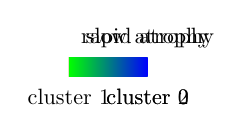
\begin{tikzpicture}[scale=1, every node/.style={scale=0.8}]
    \shade[left color=red,right color=green] (\gradLimLeft,2.5) rectangle (0,2.75);
    \shade[left color=green,right color=blue] (0,2.5) rectangle (\gradLimRight,2.75);
    \node[inner sep=0] (corr_text) at (\gradLimLeft,2.25) {cluster 0};
    \node[inner sep=0] (corr_text) at (0,2.25) {cluster 1};
    \node[inner sep=0] (corr_text) at (\gradLimRight,2.25) {cluster 2};
    \node[inner sep=0] (corr_text) at (\gradLimLeft,3) {rapid atrophy};
    \node[inner sep=0] (corr_text) at (\gradLimRight,3) {slow atrophy};
  \end{tikzpicture}
%     \caption{}
%       \label{fig:adniClust}
  \vspace{1em}
  \end{subfigure}
  
  %%%%%%%%%%%%%%%%%%% BRAINS %%%%%%%%%%%%%%5%%%%%%
  
  \begin{subfigure}[b]{0.3\textwidth}
   \centering
  \begin{tikzpicture}[scale=\scalingFactor, every node/.style={scale=1}]
    \node[inner sep=0] (image) at (0,0) {\includegraphics[width=\scalingFactorBrains\textwidth]{../images/vwdpm/blend14_adniThavgFWHM0InithistCl3Pr0Ra1_VWDPMStd.png}}; 
    \node[inner sep=0] (label) at (0,3.5) {tAD - ADNI};
  \end{tikzpicture}
%     \caption{}
%       \label{fig:adniClust}
  \end{subfigure}
   \begin{subfigure}[b]{0.3\textwidth}
  \centering
  \begin{tikzpicture}[scale=\scalingFactor, every node/.style={scale=1}]
    \node[inner sep=0] (corr_text) at (0,0) {\includegraphics[width=\scalingFactorBrains\textwidth]{../images/vwdpm/drcThavgFWHM0InithistCl3Pr0Ra1_VWDPMStdAD_blend24.png}};
    \node[inner sep=0] (label) at (0,3.5) {tAD - DRC dataset};
  \end{tikzpicture}
%     \caption{}
%       \label{fig:drcClustAD}
  \end{subfigure}
   \begin{subfigure}[b]{0.3\textwidth}
  \centering
  \begin{tikzpicture}[scale=\scalingFactor, every node/.style={scale=1}]
    \node[inner sep=0] (corr_text) at (0,0) {\includegraphics[width=\scalingFactorBrains\textwidth]{../images/vwdpm/drcThavgFWHM0InithistCl3Pr0Ra1_VWDPMStdPCA_blend24.png}};
    \node[inner sep=0] (label) at (0,3.5) {PCA - DRC dataset};
  \end{tikzpicture}
%     \caption{}
%       \label{fig:drcClustPCA}
  \end{subfigure}
  
  %%%%%%%%%%%%%%%%%%%%%% trajectories %%%%%%%%%%%%%%%%%%%%%%%
  
    \begin{subfigure}[b]{0.3\textwidth}
    \centering
%     \vspace{-2em}
    \includegraphics[width=\scalingFactorTraj\textwidth]{../images/vwdpm/trajSamplesOneFig_adniThavgFWHM0InithistCl3Pr0Ra1_VWDPMStd.png}
%     \caption{}
%       \label{fig:adniTraj}
  \end{subfigure}
      \begin{subfigure}[b]{0.3\textwidth}
    \centering
%     \vspace{-2em}
    \includegraphics[width=\scalingFactorTraj\textwidth]{../images/vwdpm/trajSamplesOneFig_drcThavgFWHM0InithistCl3Pr0Ra1_VWDPMStdAD.png}
%     \caption{}
%       \label{fig:drcTrajAD}
  \end{subfigure}
    \begin{subfigure}[b]{0.3\textwidth}
    \centering
%     \vspace{-2em}
    \includegraphics[width=\scalingFactorTraj\textwidth]{../images/vwdpm/trajSamplesOneFig_drcThavgFWHM0InithistCl3Pr0Ra1_VWDPMStdPCA.png}
%     \caption{}
%       \label{fig:drcTrajPCA}
  \end{subfigure}
  
%   \caption{}
%   \label{fig:clustTrajAll}
Marinescu et al., IPMI, 2017
\end{figure}

\textbf{Conclusion}: Model reveals spatially disconnected patterns of atrophy

\end{frame}


\begin{frame}
\frametitle{Collaboration}

Crucial to the success of my work were several aspects:

\begin{small}
\begin{columns}[T]
%     \hspace{-4em}
    \begin{column}{.47\textwidth}

     \begin{itemize}
      \item Joint supervisors from distinct fields: computer science and neurology
%       \vspace{1em}
      \begin{figure}
      \begin{subfigure}{0.42\textwidth}
      \centering
      Daniel Alexander\\
      (CMIC)
      \includegraphics[scale=0.25]{Danny-Alexander.jpeg}  
      \end{subfigure}\hspace{0.5em}\begin{subfigure}{0.42\textwidth}
	\centering
	Sebastian Crutch\\
	(BRC)
	
      \includegraphics[scale=0.27]{Seb_Crutch_photo.JPG}  
      \end{subfigure}
     \end{figure}
  
  \vspace{1em}
  
 \end{itemize}

    
%     \includegraphics[scale=1]{pondLogo.png}  
    \end{column}
    
    
    \begin{column}{.47\textwidth}
    
    \begin{itemize}
    \item Multi-disciplinary collaboration: computational center (CMIC) + clinical center (DRC)
    
    \item Understanding of the clinical workflow through the miniMD
    
    \item Supportive research group
    \includegraphics[width=0.9\textwidth,trim=0 40 0 40, clip]{MIGPOND}
    
  \end{itemize}
 
    \vspace{-2em}

    
\end{column}
\end{columns}

\vspace{1em}

I would like to thank the EPSRC and NIHR BRC for funding me

% \vspace{2em}
\begin{figure}
\centering
\includegraphics[height=1.0cm]{CDTlogo.png} \hspace{5em} \includegraphics[height=1.0cm]{epsrc_logo.jpg}\hspace{5em}\includegraphics[height=1.0cm]{brcLogo.jpg} 
   
\end{figure}


% 

\end{small}

\vspace{-2em}

\end{frame}

% \begin{frame}
% \frametitle{Acknowledgements} 
%       \vspace{2em}
% 
% 
%  
% \end{frame}
 
 
\end{document}

